Gegeben sind die Punkte $A=(-2,3,-2)$ und $B=(-6,-1,1)$. Von welchen Punkten
der $x$-Achse wird die Strecke $AB$ unter einem Winkel von $\alpha = 90^\circ$ gesehen?
\begin{center}
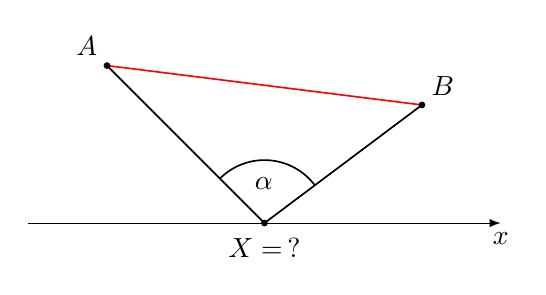
\begin{tikzpicture}[>=latex,scale=1]

\coordinate (A) at (-2,2);
\coordinate (B) at (2,1.5);
\coordinate (P) at (0,0);


\draw[semithick](P)++({0.8*cos(atan(1.5/2))},{0.8*sin(atan(1.5/2))}) arc(atan(1.5/2):atan(1.5/2)+98:0.8)node[right=9pt,yshift=-2pt]{$\alpha$};

\draw[black,->](-3,0)--++(6,0)node[below]{$x$};
\draw[semithick,red](A)--(B);
\draw[semithick](P)--(B);
\draw[semithick](A)--(P);


\draw[black,fill](A)circle(1pt)node[above left]{$A$};
\draw[black,fill](B)circle(1pt)node[above right]{$B$};
\draw[black,fill](P)circle(1pt)node[below=2pt]{$X=\,?$};

\end{tikzpicture} 
\end{center}

\thema{Zwischenwinkel}

\begin{loesung}
Die Punkte $X$ der $x$-Achse haben die Ortsvektoren
\[
\vec x=\begin{pmatrix}x\\0\\0\end{pmatrix}
.
\]
Die Vektoren $\overset{\rightarrow}{XA}$ und $\overset{\rightarrow}{XB}$ sind
genau dann senkrecht, wenn das Skalarprodukt verschwindet, also
\begin{align*}
\left(
\begin{pmatrix}-2\\3\\-2\end{pmatrix}
-
\begin{pmatrix}x\\0\\0\end{pmatrix}
\right)\cdot\left(
\begin{pmatrix}-6\\-1\\1\end{pmatrix}
-
\begin{pmatrix}x\\0\\0\end{pmatrix}
\right)
&=0
\\
\begin{pmatrix}-2-x\\3\\-2\end{pmatrix}
\cdot
\begin{pmatrix}-6-x\\-1\\1\end{pmatrix}
&=0
\\
(2+x)(6+x)-3-2&=0\\
x^2+8x+7&=0\\
(x+7)(x+1)&=0
\end{align*}
Daraus liest man ab, dass $x\in\{-1,-7\}$ sein muss, die gesuchten Punkte
sind also $(-1,0,0)$ und $(-7,0,0)$.
\end{loesung}

